\begin{frame}{Experimental Setup}
	\begin{itemize}
		\item Training
		\begin{itemize}
			\item Four benchmark domains
			\begin{itemize}
				\item {Blocks words, Navigator, IPC-grid+, Ferry}
			\end{itemize}
			\item 20 intervention problems for each domain
			\item Max 100 observation traces for each intervention problem
		\end{itemize}
		
		\item Testing
		\begin{itemize}
			\item 3 different instances of 20 intervention problems for each domain
			\item Max 10 observation traces for each intervention problem
		\end{itemize}
		
		\item Accuracy measures
			\begin{itemize}
				\item Predict intervention in testing dataset using the trained model
				\item compute True-positive, False-positive, True-negative, False-negative rates 
			\end{itemize}
	\end{itemize}
\end{frame}


\begin{frame}{Results}
	\begin{itemize}
		\item Accuracy in predicting intervention online
		\begin{itemize}
			\item Very high TPR, TNR 
			\item Very low FPR, FNR
		\end{itemize}
		\begin{figure}[p]
			\centering{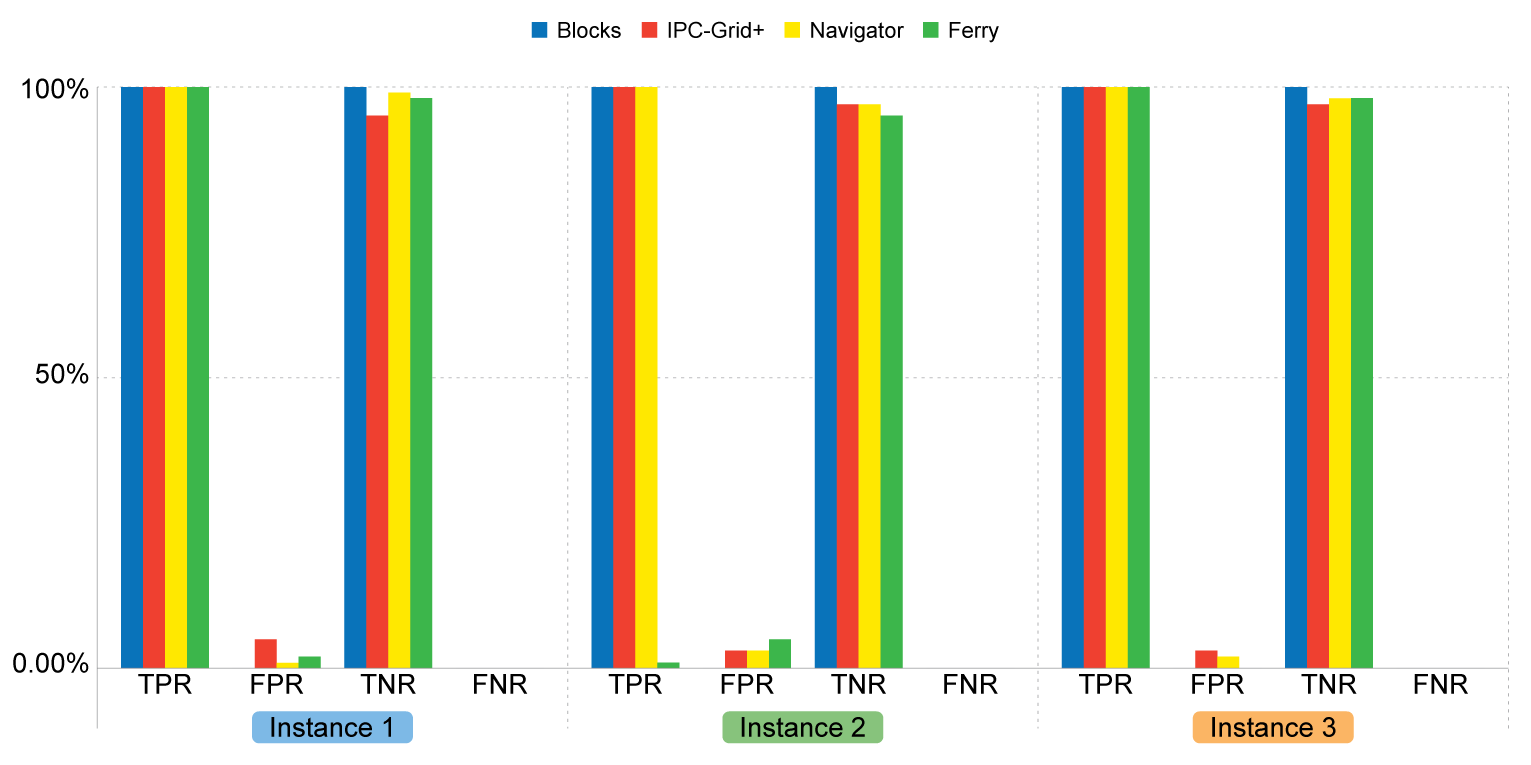
\includegraphics[width=3.5 in]{accuracy.png}}
			\label{fig:accuracy}
		\end{figure}
	\end{itemize}
\end{frame}
